\documentclass[master.tex]{subfiles}
 
\begin{document}

There are three different main problems to solve in this simulation.
\begin{itemize}
    \item Derivatives (parallel and perpendicular)
    \item Time Integration
    \item Poisson/Laplace equation solving
\end{itemize}

\subsection{Derivatives}
Since a simple grid is chosen for discretization standard finite-differences schemes are used for the derivatives and a special scheme for the Poisson brackets (Arakawa-scheme) \cite{arakawa}.\newline
These are the discretizations used throughout the simulation:\newline
\textit{Coordinates not involved are omitted for readability. $T_{i + 1} = T_i + h_T$ for T in $\{z, x, y\}$}
\begin{itemize}
    \item Perpendicular Gradient $\nabla_{\perp} = \vec{n}\cdot\nabla$\\
     \begin{small}
        \begin{equation}
        \begin{split}
            \nabla_{\perp} f(z, x_i,y_j) &\approx  \quad\frac{-f(x_{i+2},y) + 8 \cdot f(x_{i + 1}, y) -  8 \cdot f(x_{i - 1}, y) + f(x_{i - 2}, y)}{6 \cdot h_x} \\
            &\quad + \frac{-f(x,y_{i + 2}) + 8 \cdot f(x, y_{i + 1}) -  8 \cdot f(x, y_{i - 1}) + f(x, y_{i - 2})}{6 \cdot h_y}\\
            &\quad + O(h_x^4) + O(h_y^4)
        \end{split}
        \end{equation}
    \end{small}
    \item Parallel Gradient $\nabla_{\parallel} = \vec{e_z}\cdot\nabla = \partial_z$\\
    \begin{equation}
        \nabla_{\parallel} f(z_i,x,y) \approx \frac{-f(z_{i+2}) + 8 \cdot f(z_{+1}) - 8 \cdot f(z_{-1}) + f(z_{-2})}{12 \cdot h_z} + O(h_z^4)
    \end{equation}
    \item Second parallel derivative $\partial_z^2$\\
    \begin{equation}
           \partial_z^2f(z_i,x,y) \approx \frac{f(z_{i+1})-2\cdot f(z_i)+ f(z_{i-1})}{h_z^2} + O(h_z)
    \end{equation}
    \item Fourth derivative in perpendicular direction $\Delta_\perp \cdot \Delta_\perp$\\
    \begin{footnotesize}
    \begin{equation}
    \begin{split}
    \Delta_\perp^2f(z,x_i,y_j) \approx \frac{f(x_{i+2},y_j) - 4 \cdot f(x_{i+1},y_j) +6\cdot f(x_i,y_j) -4 \cdot f(x_{i-1},y_j) + f(x_{i-2}, y_j)}{h_x^4}  \\ + \frac{f(x_{i+2},y_j) - 4 \cdot f(x_{i+1},y_j) +6\cdot f(x_i,y_j) -4 \cdot f(x_{i-1},y_j) + f(x_{i-2}, y_j)}{h_y^4}  \\  + O(h_x^2) + O(h_y^2)
    \end{split}
    \end{equation}
\end{footnotesize}      %$[f(x,y),g(x,y)]_\perp = \partial_x f \partial_y g - \partial_y f \partial_x g$
    \item Poisson Bracket \\
    \begin{footnotesize}
        \begin{equation}
            \begin{split}
                [f(x,y), g(x,y)]_\perp = -\frac{1}{12h_xh_y} & [
                    (g_{i, j-1} + g_{i+1,j-1} - g_{i, j+ 1} - g_{i+1,j+1})(f_{i+1,j}-f_{i, j}) \\
                    &+ (g_{i-1,j-1}+g_{i,j-1}-g_{i-1,j+1} - g_{i,j+1})(f_{i,j}-f_{i-1,j})\\
                    &+ (g_{i+1,j}+g_{i+1,j+1}-g_{i-1,j}-g_{i-1,j+1})(f_{i,i+1}-f_{i,j})\\
                    &+ (g_{i+1,j+1}+g_{i+1,j}-g_{i-1,j-1}-g_{i-1,j})(f_{i,j}-f_{i,j-1})\\
                    &+ (g_{i+1, j} - g_{i, j + 1})(f_{i+1,j+1}-f_{i,j})\\
                    &+ (g_{i, j-1} - g_{i-1, j})(f_{i,j}-f_{i-1,j-1})\\
                    &+ (g_{i,j+1}-g_{i-1,j})(f_{i-1,j+1}-f_{i,j})\\
                    &+ (g_{i+1, j} - g_{i,j-1})(f_{i,j}-f_{i+1,j-1}) ]
            \end{split}
        \end{equation}
    \end{footnotesize}


\end{itemize}

\subsection{Time Integration - Karniadakis Scheme}
The time stepping is implemented using a Karniadakis scheme of 3rd order \cite{KARNIADAKIS1991414}.
It is applied to the density and velocity equations described in \autoref{sec:isothermalequations}.
In our case it iterates an equation of form
\begin{equation}
    \partial_t \Phi = F(\Phi) - \lambda_s
\end{equation}
where $\lambda_s$ represents sources and sinks and $n$ denotes the time step in the following way :
\begin{equation}\label{eq:karnidakis-scheme}
\begin{split}
    \Phi^{n + 1} = \quad &\frac{18}{11} \Phi^{n} - \frac{9}{11} \Phi^{n-1} + \frac{2}{11}  \Phi^{n-2}\\
     + &\frac{6}{11}\Delta t \cdot (3 \cdot F(\Phi)^{n+1} - 3 \cdot F(\Phi)^{n} + F(\Phi)^{n-1} + \lambda_s)
\end{split}
\end{equation}
This scheme has been shown to be stable at high \ac{CFL} number for the incompressible Navier-Stokes equation \cite{KARNIADAKIS1991414}.

\subsection{Poisson Equation solver}
There are two Poisson-like equations to solve. The first one is necessary to apply the Padé-approximation of the gyro-averaging operator and is solved using a Fourier decomposition. The second one is the polarization equation as described in \autoref{sec:isothermalequations} and is solved using a \ac{SOR} Gauss-Seidel-iterator.

\subsubsection{Gyro-Averaging - Fourier Solver}
The gyro-averaging operation has the form:
\begin{equation}
    \alpha \Delta U(x, y) = F(x, y)
\end{equation}
This equation is solved using Fourier-Method as it is described here \cite{fft-poisson}. To achieve a periodic function in x-direction the domain is extended in this direction before computation. The transformation rule is:
\begin{equation}
\label{eq:gyro-transformation}
\begin{split}
    t\colon [n_x, n_y] & \to [4 \cdot n_x, n_y]\\
    f(x, y) &\mapsto \begin{cases}
    \overbrace{2 f(0, y)}^{Offset} + \overbrace{(f(0, y) - f(1, y))}^{Linear \,\, Interpolation} - f(n_x - x, j) & x \leq n_x\\
    f(x - n_x, j) & n_x < x \leq 2n_x\\
    f(3n_x-x,j) & 2n_x < x \leq 3n_x \\
    2 f(0, j) + (f(0, y) - f(1, y))  - f(x - 3n_x, j) & else
    \end{cases}
\end{split}
\end{equation}
and it is visualized in \autoref{fig:fftwprofile}.
\begin{figure}[!hbtp]
    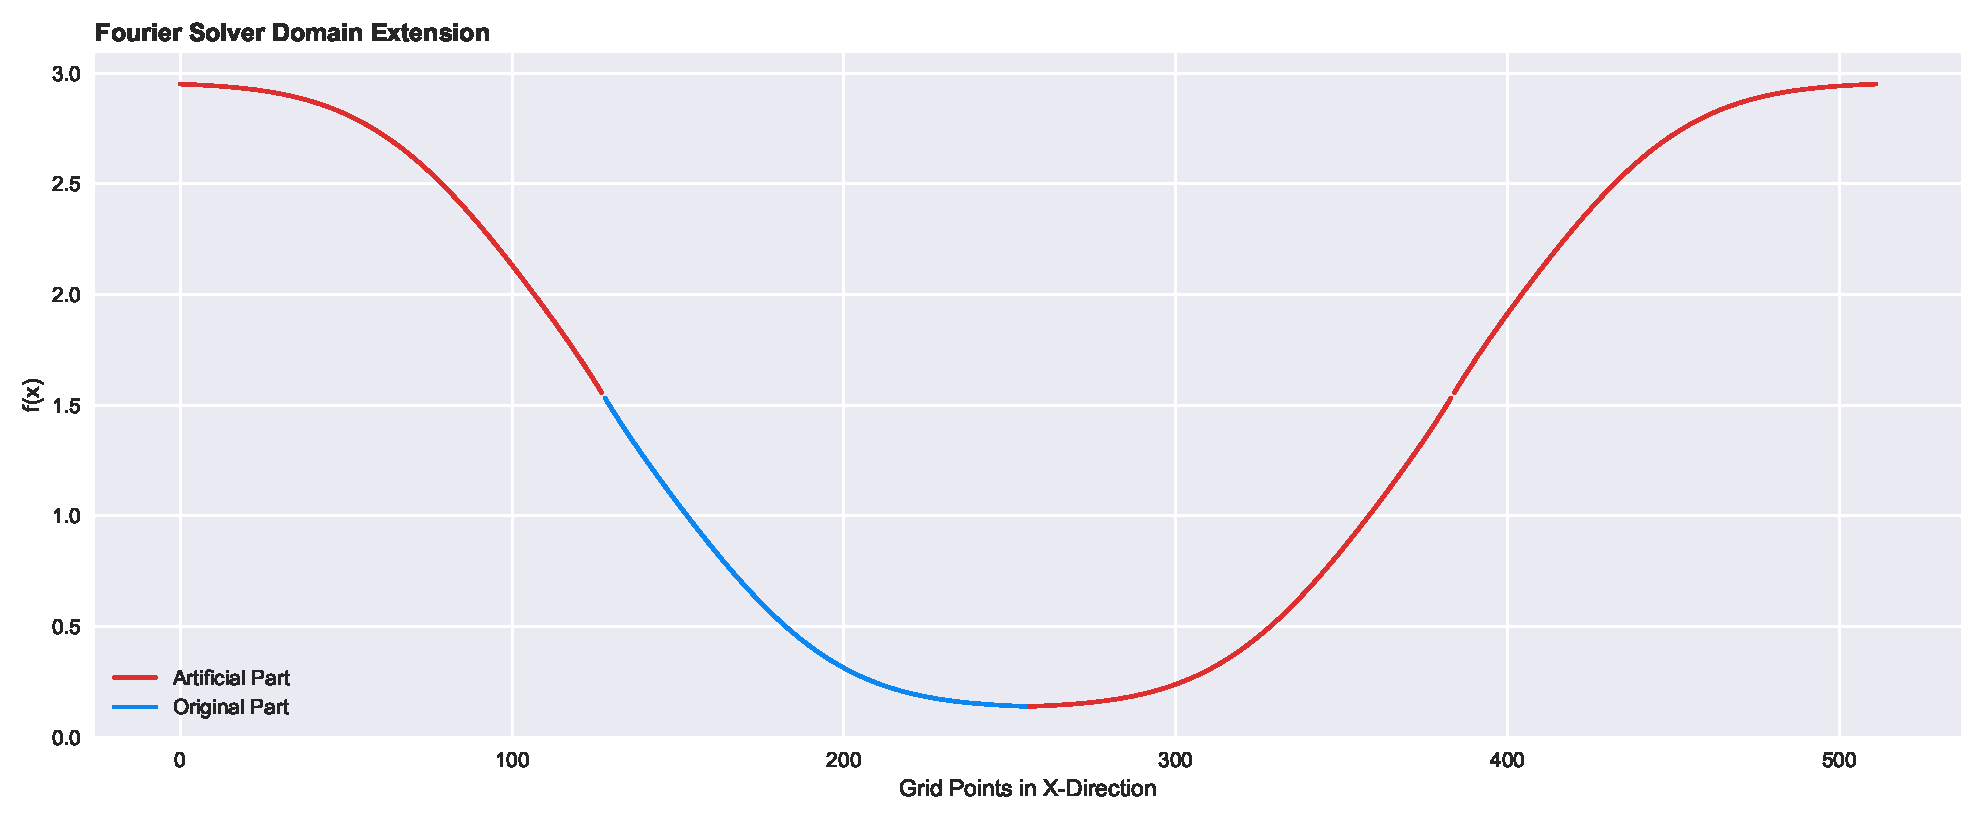
\includegraphics[width=\linewidth]{pdfs/fftwextension.pdf}
    \caption{Profile of domain extension for Fourier Solver.}
    \label{fig:fftwprofile}
\end{figure}

This artificially creates a periodic function which should reduce numerical artifacts from the solver.

\subsubsection{Polarization Equation - \ac{SOR} Gauss Seidel Iterator} \label{sec:polarization-equation}
The polarization equation (\autoref{eq:polarization}) has the form:
\begin{equation}
    \nabla\left( A(x, y) \nabla U(x, y)\right) = F(x, y)
\end{equation}
The discretization is presented here \cite{DielectricPoisson}. The problem solved in the reference evolves from the variable dielectric Poisson equation which is of a similar form. To solve the linear system a \ac{SOR} iterator is implemented which is further described here \cite{SORPaper}. Implementation details are presented in \autoref{sec:sor-solver-implementation}.

\subsection{Choosing viscosities}
The viscosities involved in the evolution equations are fundamental for the convergence of the simulation. Currently we only have a heuristic approach for finding appropriate values.\newline
The \textit{quality} of the viscosities is derived from turbulence spectra of the densities, parallel velocities, potential and vorticity. Good parameters show the characteristic turbulence spectrum of energy dissipation via an energy cascade \cite{TurbulentSpectra}.\newline
Viscosities that are to high give rise to artificial waves and eddies in the length scale of the distance between grid points and/or block the full development of an energy cascade. On the other hand viscosities that are too low hinder the full dissipation of smaller eddies which then in turn never completely decay. Since they are in length scale of grid distances they cannot be resolved sufficiently by the simulation and thus result into unwanted artificial artifacts.

\end{document}